% *********************************************************************
% © 2021–2026 Jeremy Sylvestre
%
% Permission is granted to copy, distribute and/or modify this document
% under the terms of the GNU Free Documentation License, Version 1.3 or
% any later version published by the Free Software Foundation; with no
% Invariant Sections, no Front-Cover Texts, and no Back-Cover Texts. A
% copy of the license is included in the appendix entitled “GNU Free
% Documentation License” that appears in the output document of this
% PreTeXt source code. All trademarks™ are the registered® marks of
% their respective owners.
%
% *********************************************************************

\newcommand*{\xmin}{0.5}
\newcommand*{\xmax}{5.5}
\newcommand*{\ymin}{-2.5}
\newcommand*{\ymax}{4.5}
\newcommand*{\func}{\x * \x * \x - 9 * \x * \x + 23 * \x - 14}

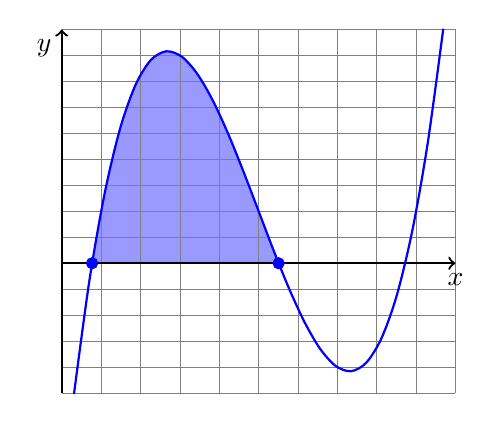
\begin{tikzpicture}
[
	closedpt/.style={circle,draw,fill,inner sep=0pt,minimum size=4pt},
	openpt/.style={circle,draw,inner sep=0pt,minimum size=4pt},
	yscale=0.66
]

	\fill[blue!40!white]
	  plot[domain=0.885:3.254, smooth] (\x,{\func})
	  -- (0.885,0)
	;

	% grid
	\foreach \x in {0.5,1,1.5,...,5.5} {
		\draw[very thin,gray] (\x,\ymin) -- (\x,\ymax);
	}
	\foreach \y in {-2.5,-2,-1.5,...,4.5} {
		\draw[very thin,gray] (\xmin,\y) -- (\xmax,\y);
	}

	% axes
	\draw[->,thick] (\xmin,0) -- (\xmax,0) node[below] {$x$};
	\draw[->,thick] (0.5,\ymin) -- (0.5,\ymax) node[below left] {$y$};

	% example graph
	\draw[thick, blue, domain=0.655:5.345, smooth] plot (\x,{\func});

	% example points
	\node[blue,closedpt] at (0.885,0) {};
	\node[blue,closedpt] at (3.254,0) {};

\end{tikzpicture}
